\documentclass{article}
\usepackage{hyperref}
\usepackage[T1]{fontenc}
\usepackage{graphicx}
\usepackage[a4paper,margin=20mm]{geometry}

\hypersetup{
    colorlinks=true,
    linkcolor=blue,
    filecolor=blue,      
    urlcolor=blue,
    pdftitle={Combined Installation Guide - Data Translation},
    pdfpagemode=FullScreen,
    pdfauthor={Rukai, Rio, Matilde},
}

\setlength\emergencystretch{\hsize}\hbadness=10000

\begin{document}
    \title{Getting started: Using Data Translation devices with Matlab}
    \author{Rukai, Rio, Matilde}
    \date{Last updated by Matilde on March 31, 2026}
    \maketitle
    
    This document outlines the installation steps to enable the use of Data Translation devices from Matlab. The files required for the installation can be found in the folder containing this installation guide.

    \section{Installation for Recent Matlab Versions}
    \textit{Note: This section is for recent Matlab versions (i.e., 2023b for instance) on recent Windows (10 or after).}

    \begin{enumerate}
        \item Register for a Mathworks account using your <username>.unimeb.edu.au or <username>.student.unimelb.edu.au email address.
        \item Right-click on \href{./matlab_R2023b_win64.exe}{{matlab\textunderscore R2023b\textunderscore win64.exe}} and click Install/Run as Administrator to install Matlab (see figure \ref{fig:matlabInstlationEg}). Note that 2023b is the latest version, where I could successfully configure the Data Translation board to work (an older version than 2023b might also work). There seems to be an issue with version 2024a recognising the board, which I was not able to resolve.
        \begin{figure}[h]
            \centering
            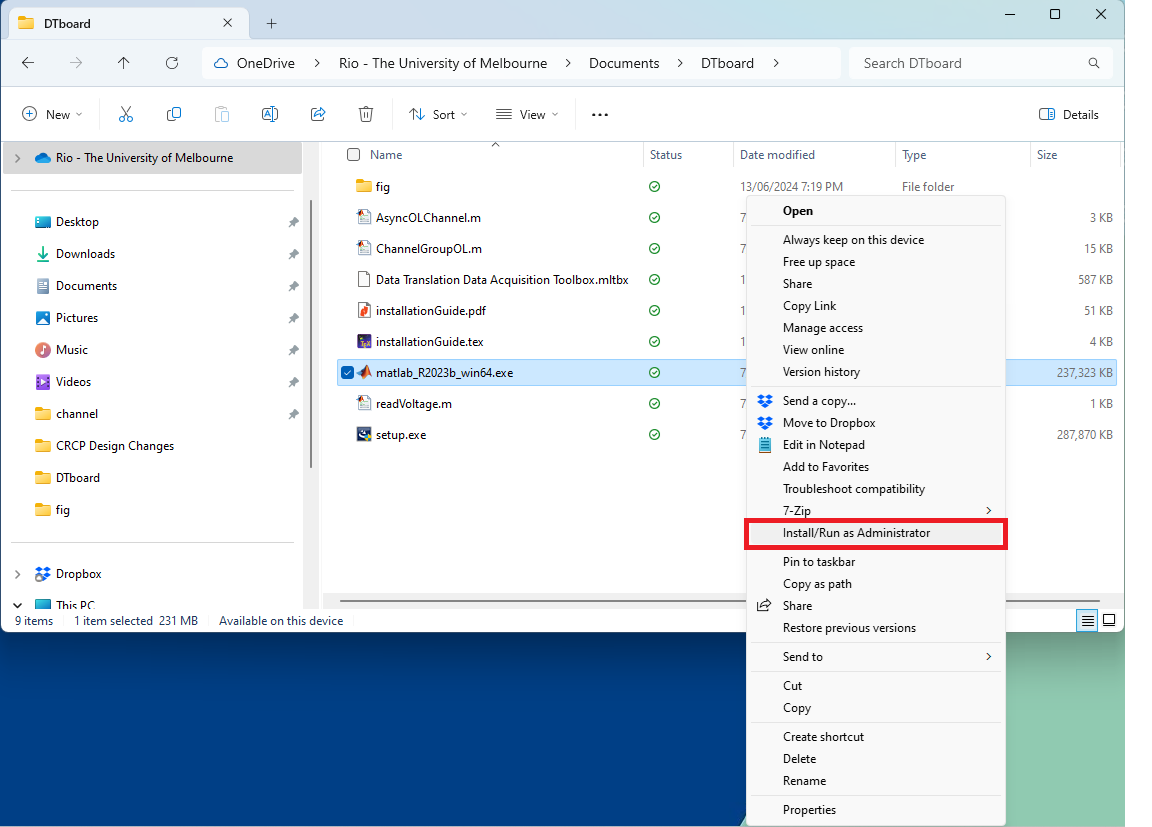
\includegraphics[scale=0.35]{fig/installMatlab.png}
            \caption{Run the Matlab installation executable as administrator.}
            \label{fig:matlabInstlationEg}
        \end{figure}

        \item Obtain the Matlab license using your Mathworks account.

        \item \label{step:openLayers}Right-click on \href{./setup.exe}{setup.exe} and click Install/Run as Administrator to install the DT-Open Layers for .NET. Note that the DT-Open Layers executable in the folder is not the latest version, since that version has a bug leading to issue using analogue output. Verify that the DT-Open Layers version is 7.8.2 as shown in figure \ref{fig:openLayerVer}.
        \begin{figure}[h]
            \centering
            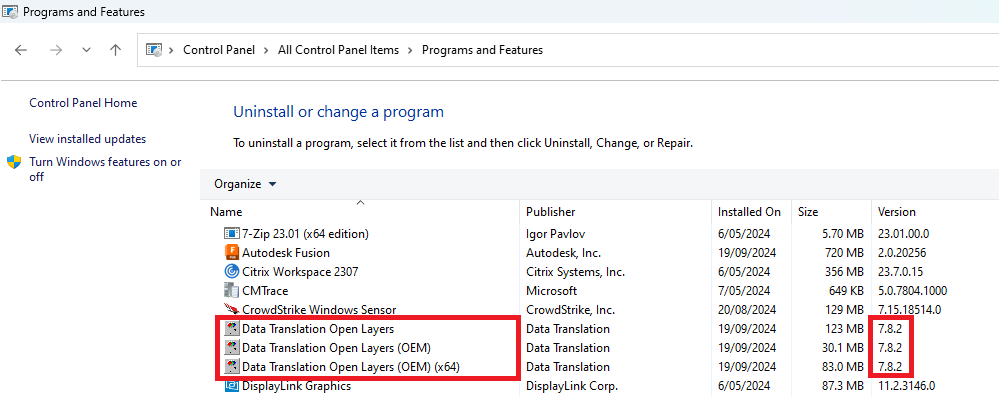
\includegraphics[scale=0.45]{fig/openLayerVer.png}
            \caption{Verify that the DT-Open Layers version is 7.8.2.}
            \label{fig:openLayerVer}
        \end{figure}

        \item Right-click on \href{./dotNetFx40_Full_x86_x64.exe}{dotNetFx40\_Full\_x86\_x64.exe} and click Install/Run as Administrator. Ensure that dotNet 4.0 or higher is installed on your computer.

        \item You will need to ask IT for permission to enable the Data Translation driver if you have a new Lenovo laptop with Windows 11. If you have an older HP laptop with Windows 10, you can ignore this step and go to \ref{step:verifyDriver}.
        \begin{enumerate}
            \item Ask IT to disable Memory integrity in Core isolation as shown in figure \ref{fig:coreIsolation}. To disable the Memory integrity the IT administrator will need to their ua account e.g. 9770ua-gromic@unimelb.edu.au. If you have trouble disabling the Memory integrity, you can contact Gogi from IT on 0466554029. He was the one who resolved the issue for me. The ticket number of my request was INC1734781.
        \end{enumerate}
        \begin{figure}[h]
            \centering
            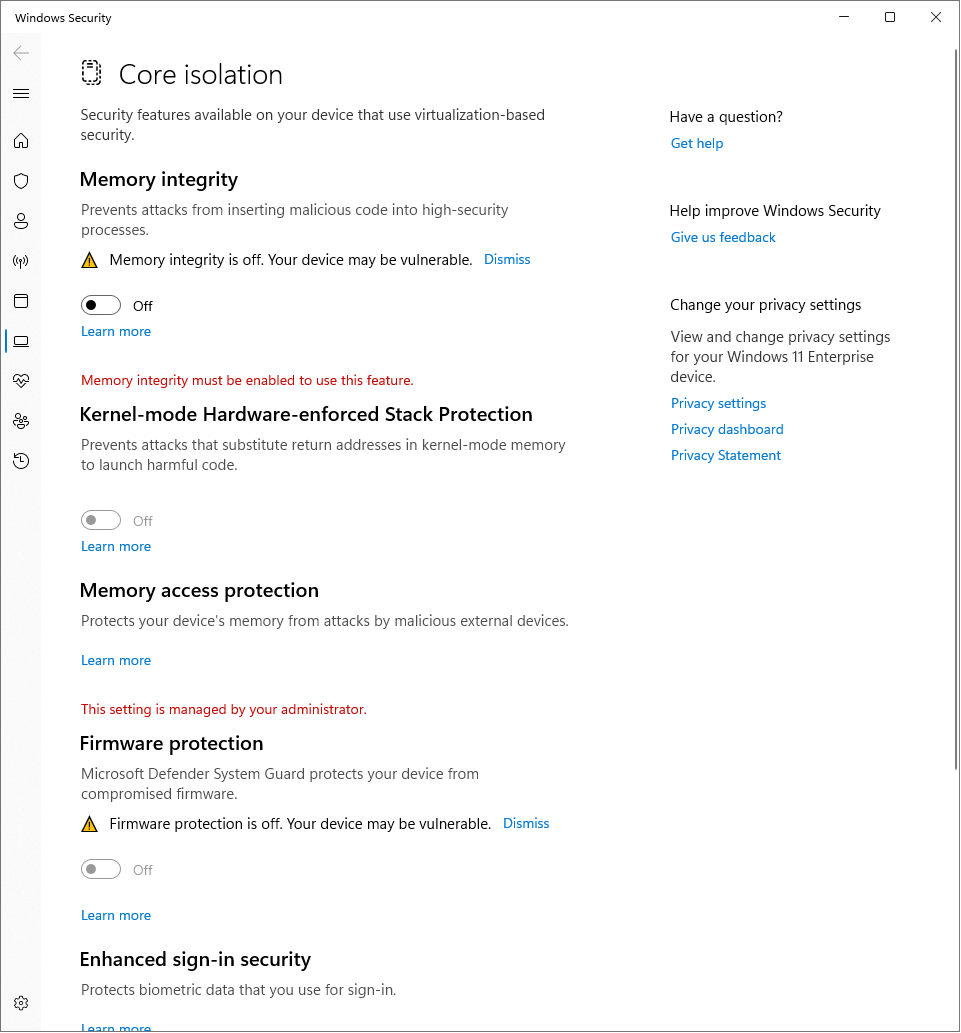
\includegraphics[scale=0.4]{fig/memoryIntegrity.png}
            \caption{Ask IT to disable Memory integrity in Core isolation for Windows 11.}
            \label{fig:coreIsolation}
        \end{figure}

        \item \label{step:verifyDriver}Connect the Data Translation device and go to the device manager. Verify that the driver is correctly installed by checking that there is no exclamation mark next to the Data Translation device, as shown in figure \ref{fig:deviceManager}.
        \begin{figure}[h]
            \centering
            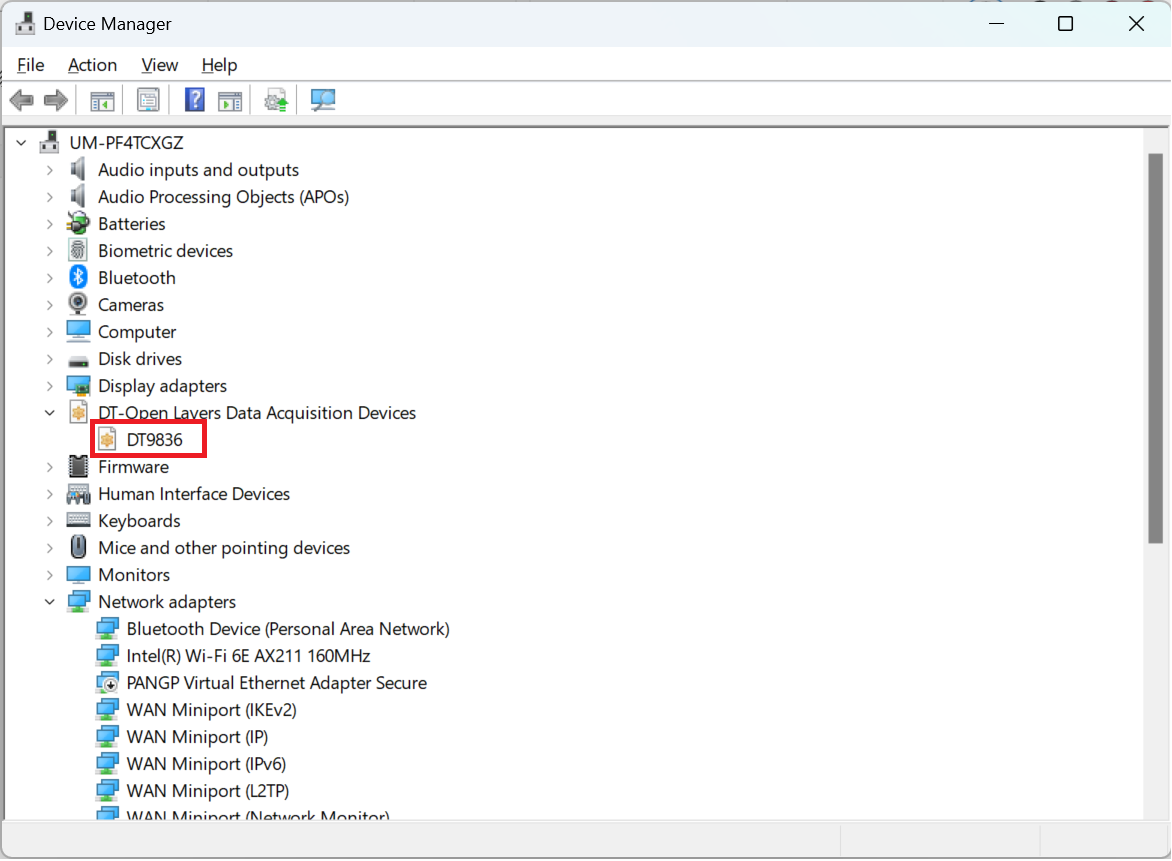
\includegraphics[scale=0.5]{fig/deviceManager.png}
            \caption{Verify that the driver is correctly installed in Device Manager.}
            \label{fig:deviceManager}
        \end{figure}

        \item Open \href{./Data Translation Data Acquisition Toolbox.mltbx}{Data Translation Data Acquisition Toolbox.mltbx} using Matlab to install the Data Translation Matlab adapter.

        \item Close and reopen Matlab. Type daqvendorlist on the command window. Verify that you see Fullname \{`Data Translation'\} for ID ``dt'' as shown in figure \ref{fig:daqvendorlist}.
        \begin{figure}[h]
            \centering
            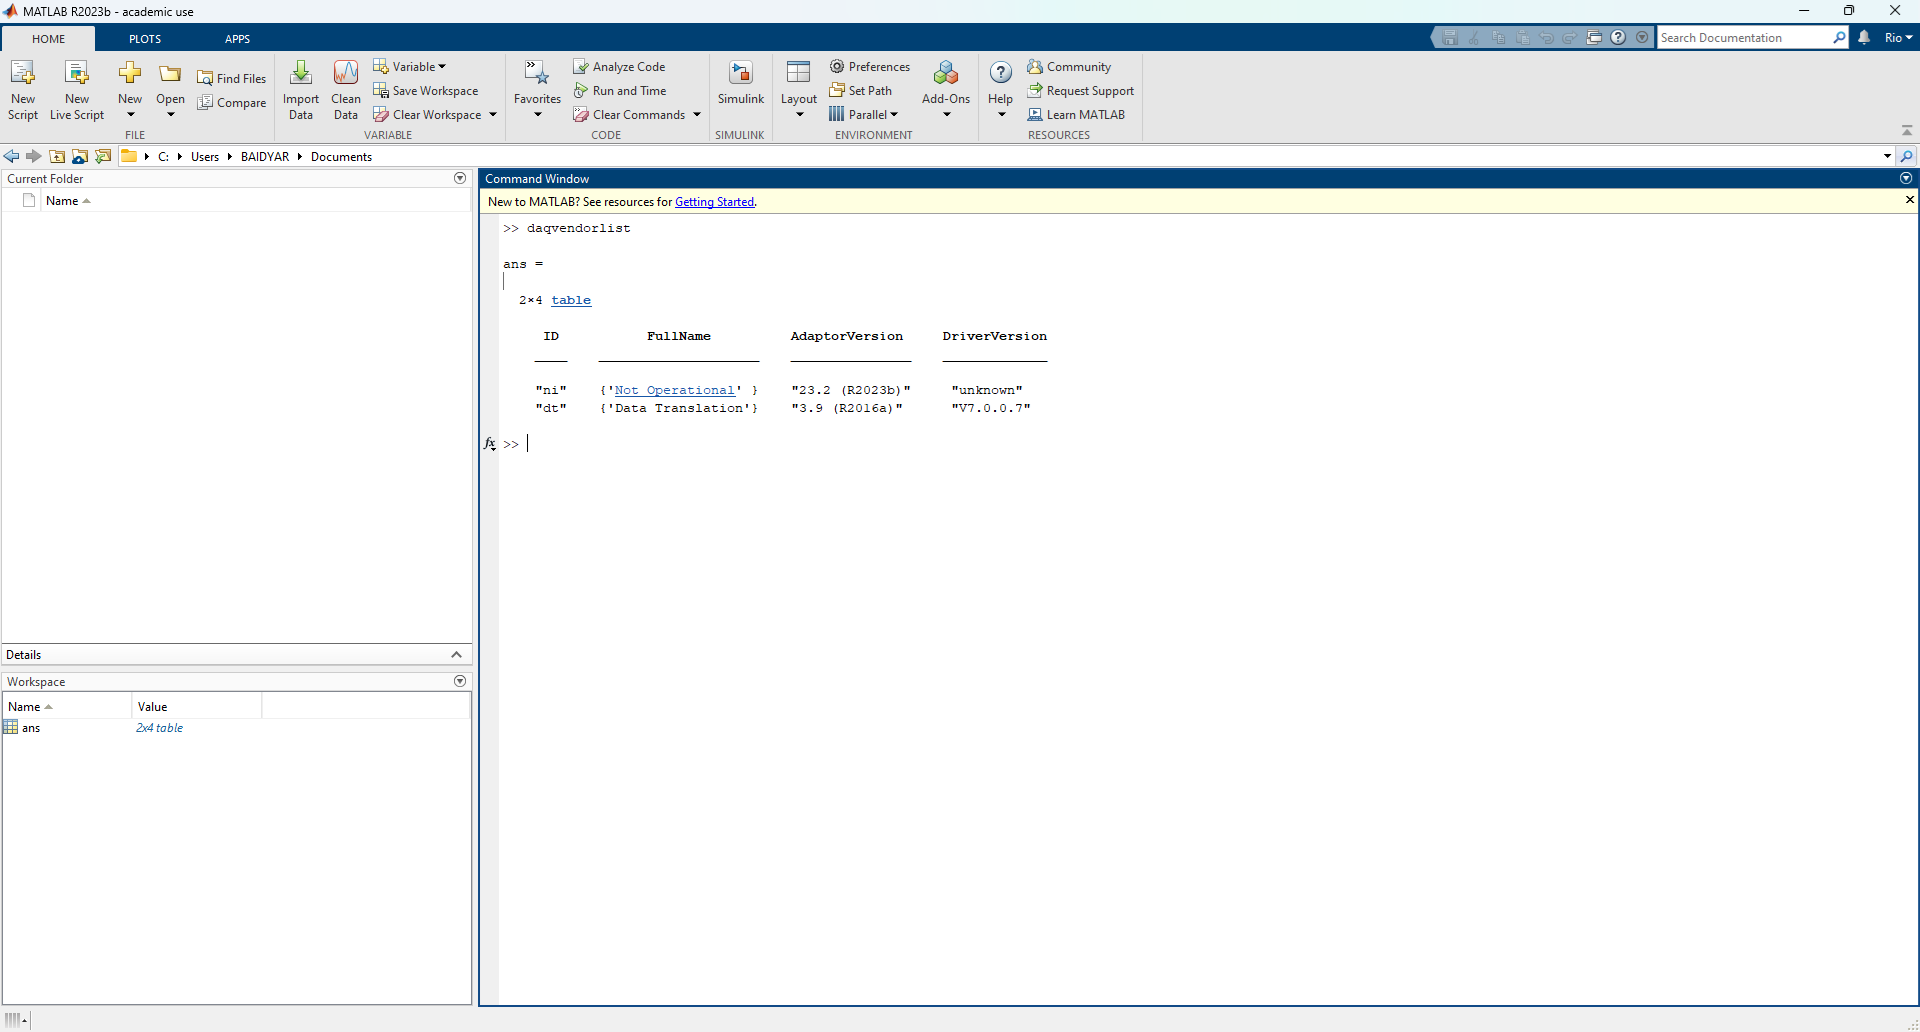
\includegraphics[scale=0.6]{fig/daqvendorlist.png}
            \caption{Verify that the Data Translation adapter is installed in Matlab.}
            \label{fig:daqvendorlist}
        \end{figure}

        \item \label{step:replaceMfile}Copy \href{./ChannelGroupOL.m}{AsyncOLChannel.m} and \href{./ChannelGroupOL.m}{ChannelGroupOL.m} from the folder containing this installation guide and replace the existing .m files in the folder C:$\backslash$Users$\backslash$<username>$\backslash$AppData$\backslash$Roaming$\backslash$MathWorks$\backslash$\mbox{MATLAB~Add-Ons}$\backslash$Toolboxes$\backslash$Data Acquisition Toolbox Support Package for Data Translation Hardware$\backslash$+daq$\backslash$+dt$\backslash$+internal (e.g. figure \ref{fig:folderLoc}). \textbf{IMPORTANT:} This path is hidden when going to users. When going to Users, I needed to type the \texttt{\textbackslash AppData} part to de-hidden it.
        \begin{figure}[h]
            \centering
            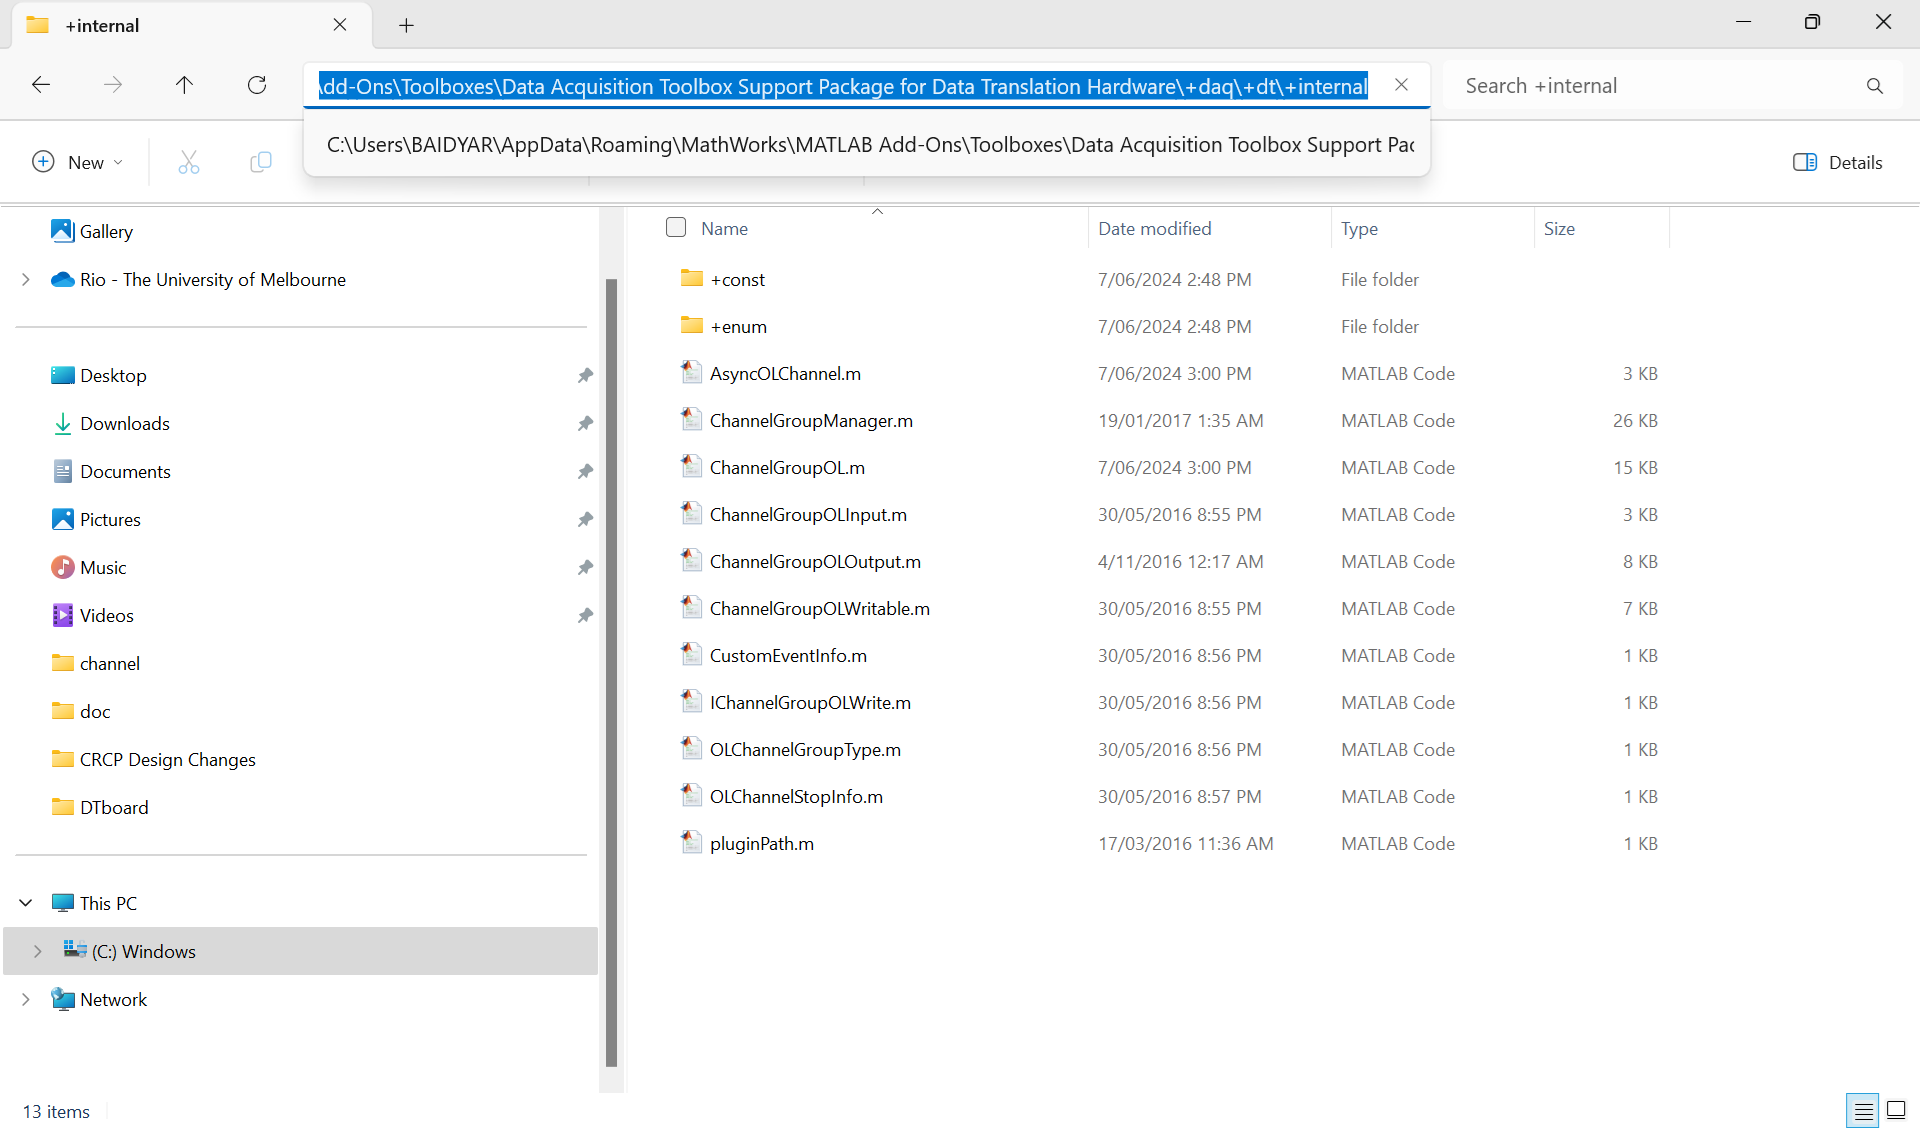
\includegraphics[scale=0.4]{fig/folderLoc.png}
            \caption{Location of the internal support files that need to be replaced.}
            \label{fig:folderLoc}
        \end{figure}

        \item Run \href{./readVoltage.m}{readVoltage.m} from the folder containing this installation guide and verify that the code does not error out and that the analogue input is working. An error message as shown in figure \ref{fig:matlabError} indicates that the replacement of the .m files in step \ref{step:replaceMfile} were incorrectly implemented.
        \begin{figure}[h]
            \centering
            \includegraphics[scale=0.35]{fig/matlaberror.png}
            \caption{Matlab error indicating incorrect replacement of the support files.}
            \label{fig:matlabError}
        \end{figure}

        \item Connect the analogue output channel 0 to an oscilloscope. Run \href{./genSineWave.m}{genSineWave.m} and verify that the sine wave is correctly generated. If a constant $-10$V is observed ensure that the Open Layers version installed is 7.8.2 (see step \ref{step:openLayers}).
    \end{enumerate}

    \newpage

    \section{SIWWI PC Installation: Attempts and Observations}
    \textit{Note: I did not achieve the installation on this PC; these are only attempts at the moment. The SIWWI PC runs Windows 7 and Matlab 2012a, and this old Matlab version is unfortunately not compatible with Data Translation. My suggestion would be to use another laptop or install more recent WIndows (reuired for recent Matlab)  and Matlab 2023 on SIWWI's PC.}

    \begin{itemize}
        \item \textbf{Constraints:}
        \begin{itemize}
            \item Data Translation (DT) requires Matlab 2023b for full modern support, which in turn requires a recent version of Windows. Windows 7 cannot handle Matlab 2023b.
            \item An internet connection on the SIWWI PC would make life significantly easier for driver validation and file transfers.
        \end{itemize}

        \item \textbf{Attempts:}
        \begin{itemize}
            \item Attempted to use the legacy executable \texttt{setup-dtbox-matlab-2026.exe}. When asked to create backups of replaced files, "No" was selected.
            \item Verification of hardware recognition was attempted by typing \texttt{daqhwinfo('dtol')} in the command window. Recognition is indicated if the \texttt{InstalledBoardIds} field displays \texttt{'0'}.
            \item For this version (R2012a), the internal support files must be replaced at this path: \\ \texttt{C:$\backslash$Program Files (x86)$\backslash$MATLAB$\backslash$R2012a$\backslash$toolbox$\backslash$daq$\backslash$daq$\backslash$+daq$\backslash$+dt$\backslash$+internal}.
            \item Scripts \texttt{read\_input.m} and \texttt{readVoltage.m} were modified to fit Matlab 2012a syntax. They can be found in the folder 'Codes for Matlab 2012'.
            \item Success check for input: If a plot figure appears showing a signal, the PC is communicating with the DT hardware.
            \item Success check for output: Connect an oscilloscope to \textbf{DAC 0} and run \texttt{generate\_output\_sine.m} to confirm if the Digital-to-Analogue path is functional.
        \end{itemize}
    \end{itemize}

\end{document}